%% Default Latex document template
%%
%%  blake@rcs.ee.washington.edu

\documentclass[letterpaper]{article}

% Uncomment for bibliog.
\bibliographystyle{unsrt}

\usepackage{graphicx}
\usepackage{lineno}
\usepackage{amsmath}

%\usepackage{fancyhdr}

%%%%%%%%%%%%%%%%%%%%%%%%%%%%%%%%%%%%%%%%5
%
%  Set Up Margins

%%%%%%%%%%%%%%%%%%%%%%%%%%%%%%%%%%%%%%%%%%%%%%%%%
% include file for:
%      Critical Page setup dimensions
%            DO NOT MODIFY
%       (for help see "Latex Line by Line" p 260)
%
\setlength\oddsidemargin{0in}
\setlength\evensidemargin{0in}

\usepackage[left=0.98in, right=0.98in, top=1.0in, bottom=1.0in]{geometry}

% %Top Margin and header
% \setlength\voffset{-0.94in}
% \setlength\topmargin{0.25in}
% \setlength\headheight{0.25in}
% %\setlength\headwidth{6.5in}
% \setlength\headsep{0.25in}
% %Body
% \setlength\textwidth{6.5in}
% \setlength\textheight{9.50in}
% %Footer
% %\setlength\footheight{0.5in}
% \setlength\footskip{0.3750in}
% Line spacing for 6 lines per inch
\linespread{0.894}  % 1.0 = single    1.6 = double
%
%          END of Critical Page Setup Dimensions
%%%%%%%%%%%%%%%%%%%%%%%%%%%%%%%%%%%%%%%%%%%%%%%%%%%

%%%%%%%%%%%%%%%%%%%%%%%%%%%%%%%%%%%%%%%%%%%%%%%%%%%
%
% Useful style and math macros
%


\newcommand\Dfrac[2]{\frac{\displaystyle #1}{\displaystyle #2}}
\newcommand\beq{\begin{equation}}
\newcommand\eeq{\end{equation}}

\newcommand\bmat{\begin{bmatrix}}
\newcommand\emat{\end{bmatrix}}

\newenvironment{solution}
{\ttfamily \vspace{0.155in} {\bf SOLUTION:} \\ }
{ \vspace{0.25in} \par }



%
%        Font selection
%
%\renewcommand{\rmdefault}{ptm}             % Times
%\renewcommand{\rmdefault}{phv}             % Helvetica
%\renewcommand{\rmdefault}{pcr}             % Courier
%\renewcommand{\rmdefault}{pbk}             % Bookman
%\renewcommand{\rmdefault}{pag}             % Avant Garde
%\renewcommand{\rmdefault}{ppl}             % Palatino
%\renewcommand{\rmdefault}{pch}             % Charter


%%%%%%%%%%%%%%%%%%%%%%%%%%%%%%%%%%%%%%%%%%%%%%%%%
%
%         Page format Mods HERE
%
%Mod's to page size for this document
\addtolength\textwidth{0cm}
\addtolength\oddsidemargin{0cm}
\addtolength\headsep{0cm}
\addtolength\textheight{0cm}
%\linespread{0.894}   % 0.894 = 6 lines per inch, 1 = "single",  1.6 = "double"

% header options for fancyhdr

%\pagestyle{fancy}
%\lhead{LEFT HEADER}
%\chead{CENTER HEADER}
%\rhead{RIGHT HEADER}
%\lfoot{Hannaford, U. of Washington}
%\rfoot{\today}
%\cfoot{\thepage}



% Make table rows deeper
%\renewcommand\arraystretch{2.0}% Vertical Row size, 1.0 is for standard spacing)

\begin{document}
\begin{centering}
{\Large  Supplemental Data: Simulation of Everting Tube Experiments}

Blake Hannaford

\today

\end{centering}

\section{Simulation Results: 8 everting tube experiments}
Each figure illustrates the results of the simulation and parameter tuning process described in the main paper, Section X.X.X.
\vspace{0.5in}

\begin{figure}[h]\centering
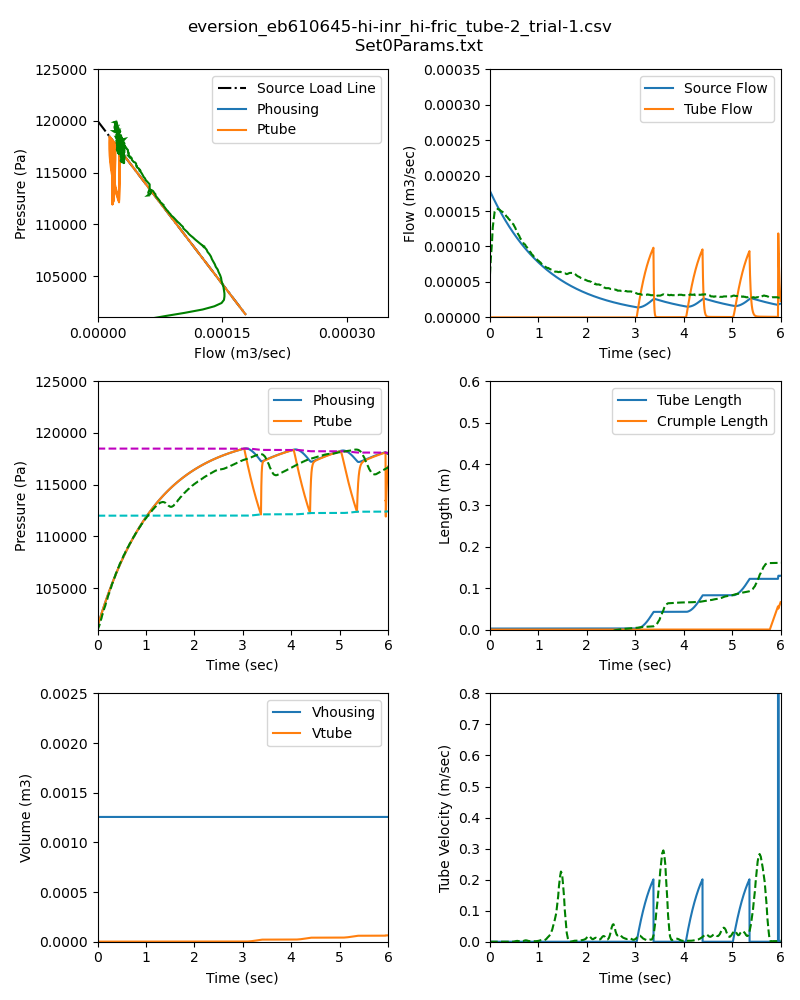
\includegraphics[width=0.475\textwidth]{Set0result27-Jul.png}
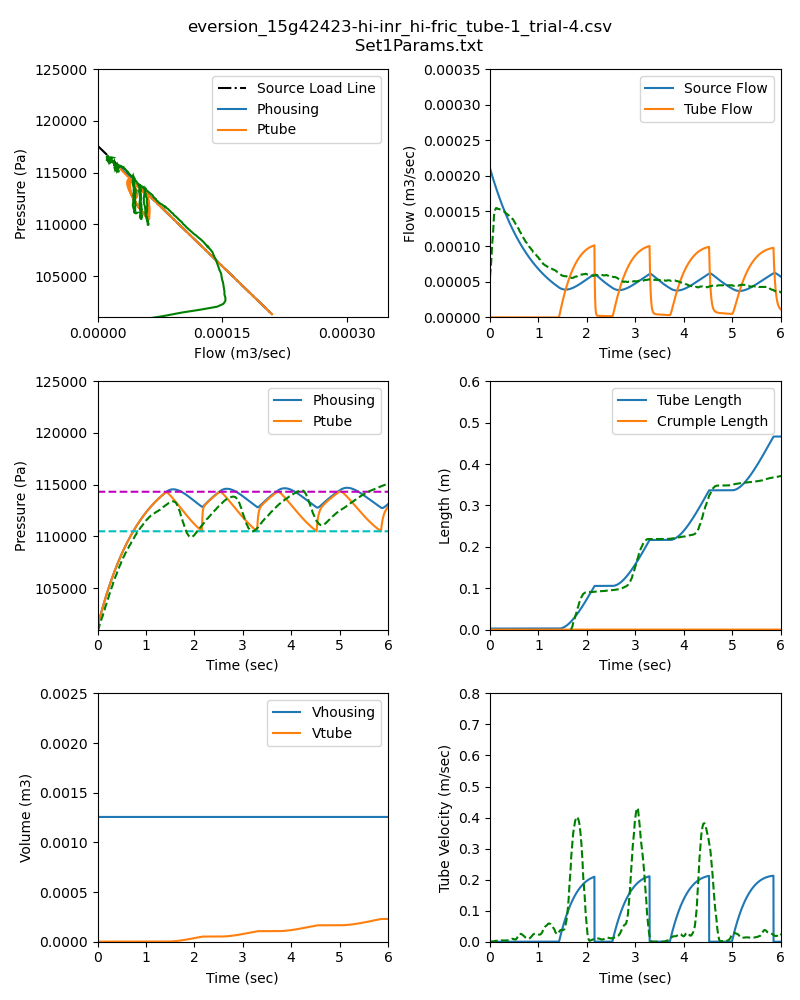
\includegraphics[width=0.475\textwidth]{Set1result27-Jul.png}
\caption{Simulations 0 and 1.}
\end{figure}

\clearpage
\begin{figure}\centering
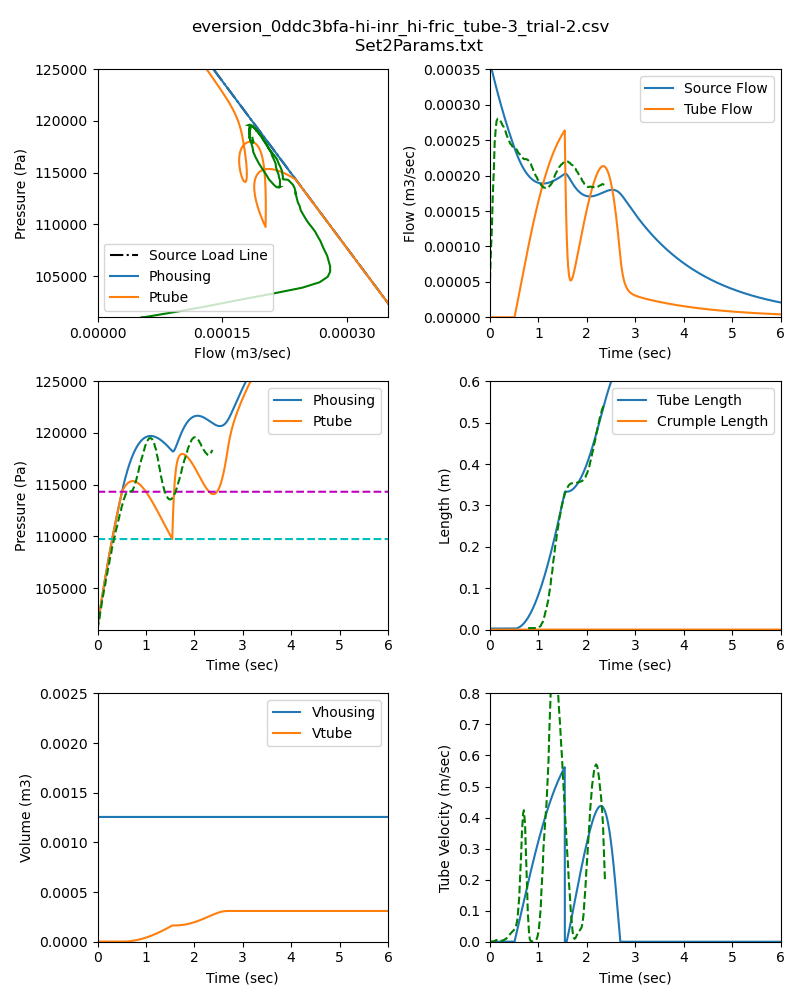
\includegraphics[width=0.475\textwidth]{Set2result27-Jul.png}
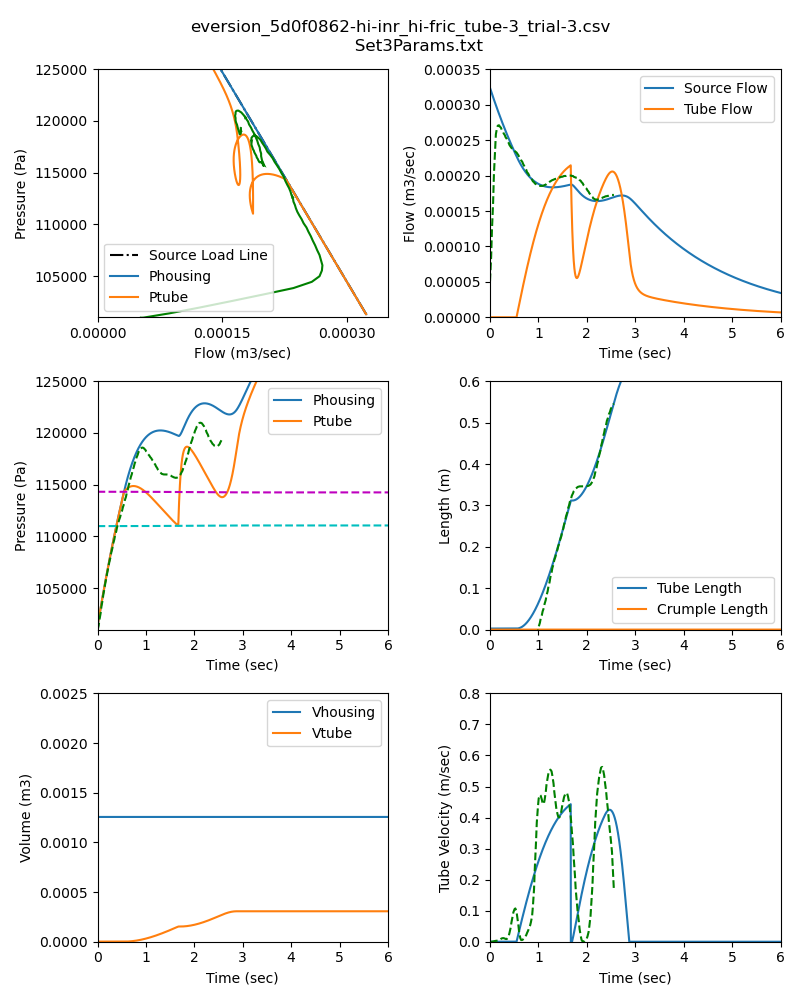
\includegraphics[width=0.475\textwidth]{Set3result27-Jul.png}
\caption{Simulations 2 and 3.}
\end{figure}


\begin{figure}\centering
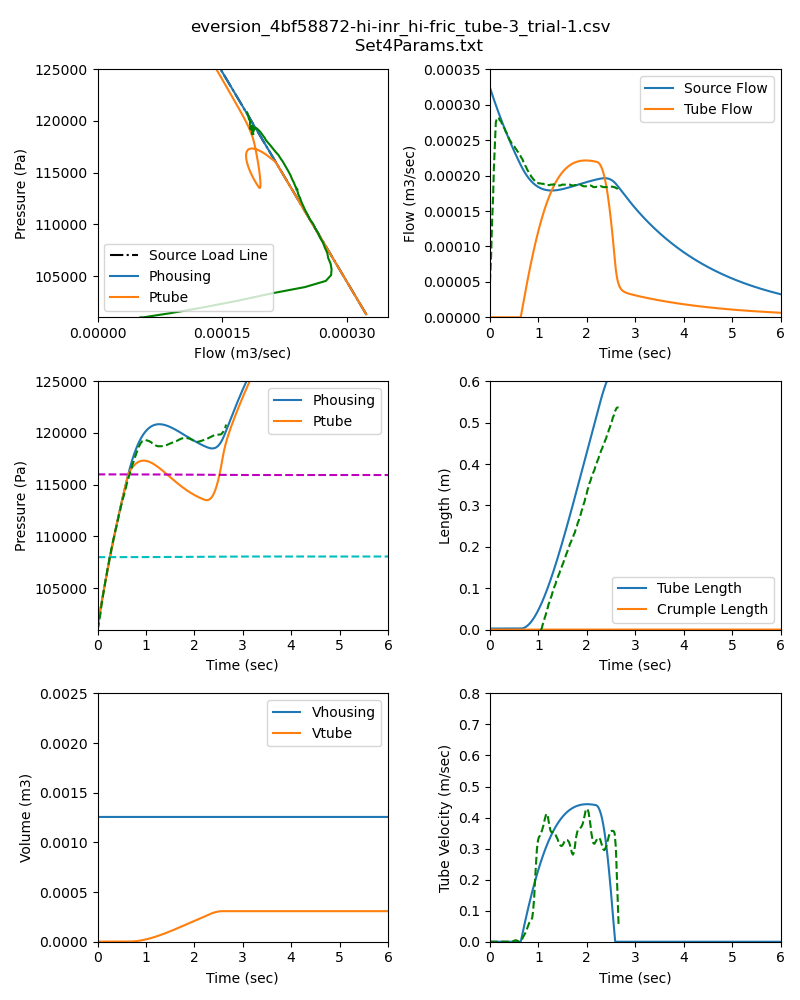
\includegraphics[width=0.475\textwidth]{Set4result27-Jul.png}
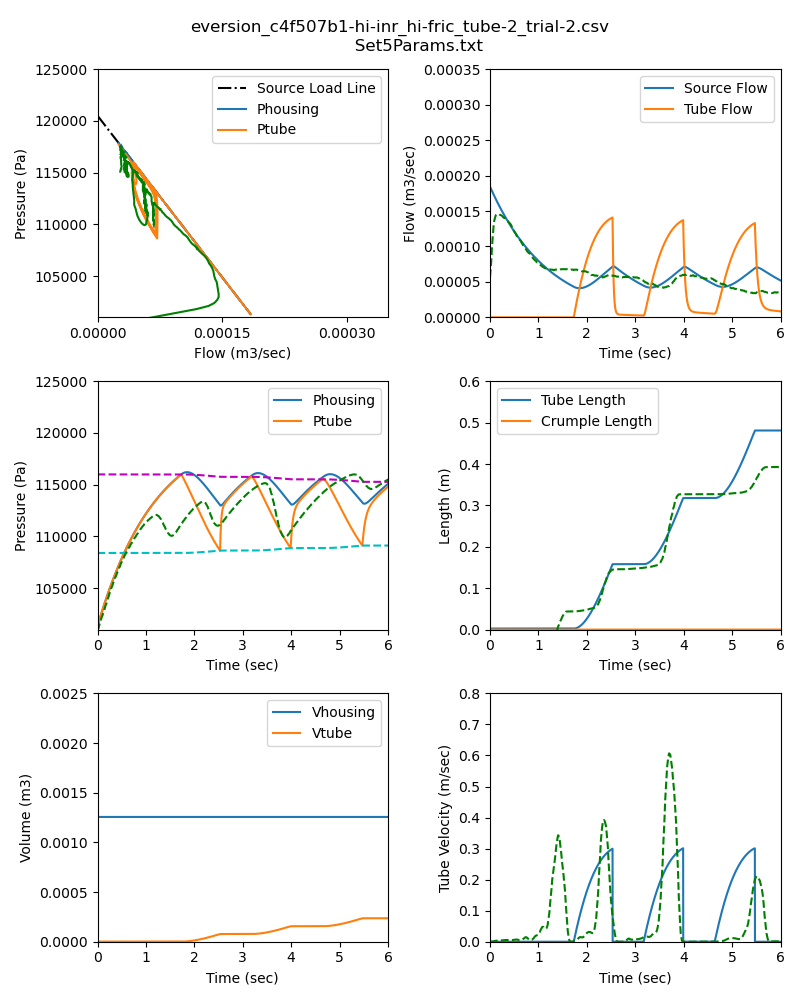
\includegraphics[width=0.475\textwidth]{Set5result27-Jul.png}
\caption{Simulations 4 and 5.}
\end{figure}


\begin{figure}\centering
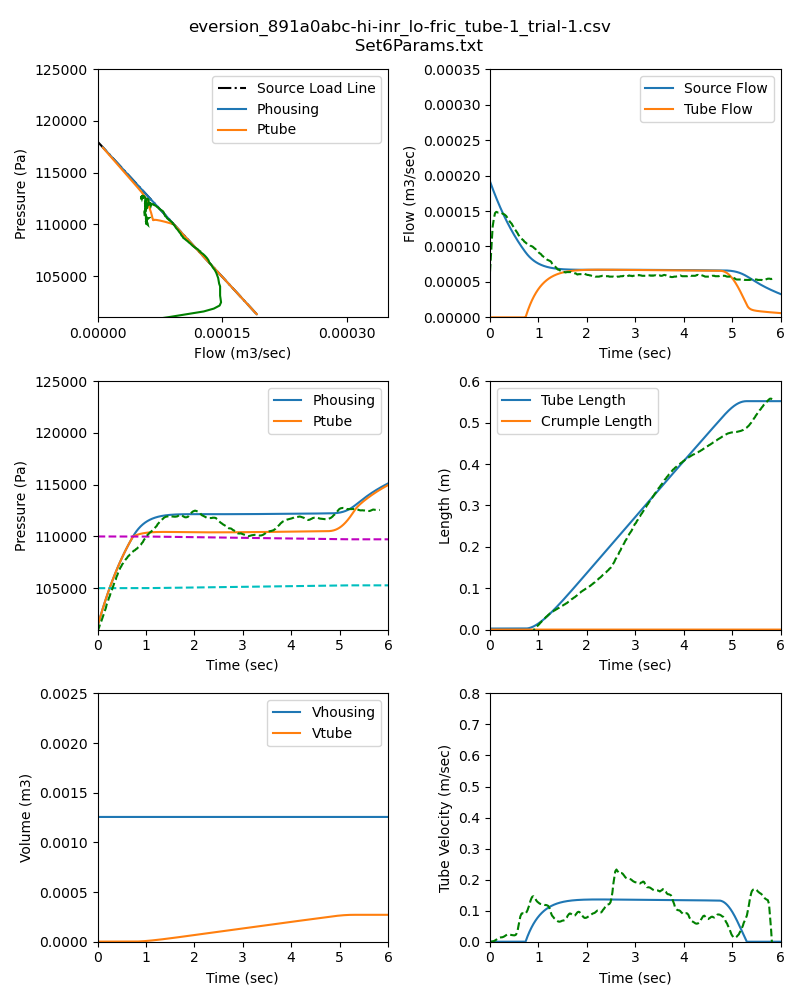
\includegraphics[width=0.475\textwidth]{Set6result27-Jul.png}
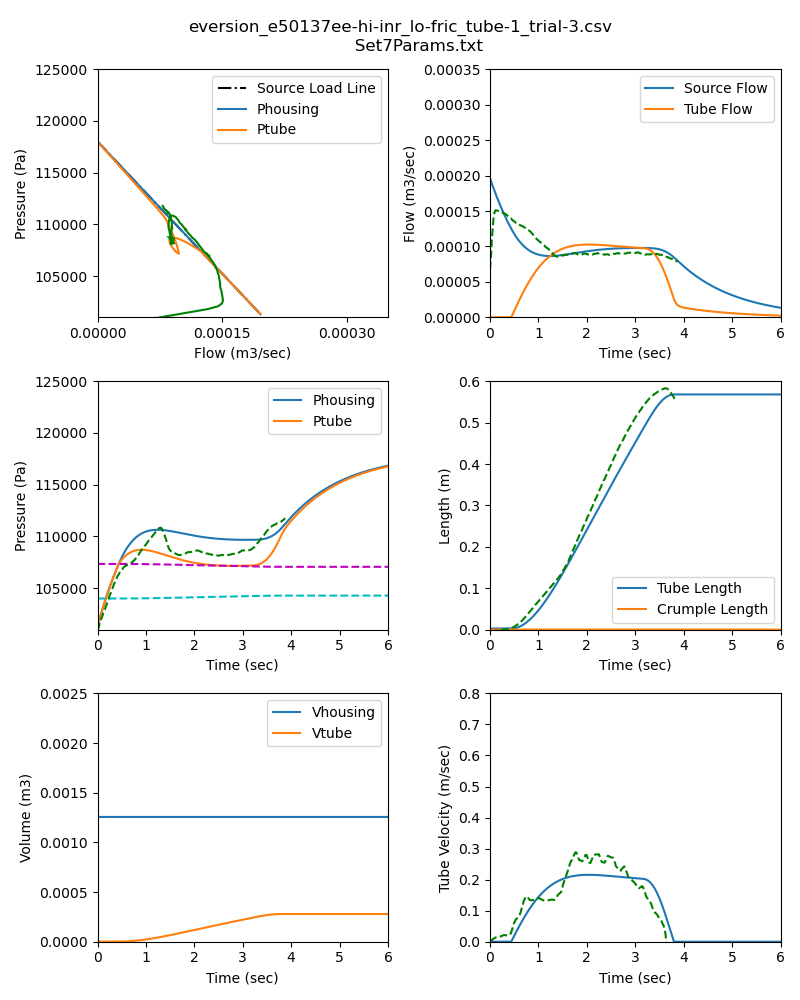
\includegraphics[width=0.475\textwidth]{Set7result27-Jul.png}
\caption{Simulations 6 and 7.}
\end{figure}



\begin{figure}\centering
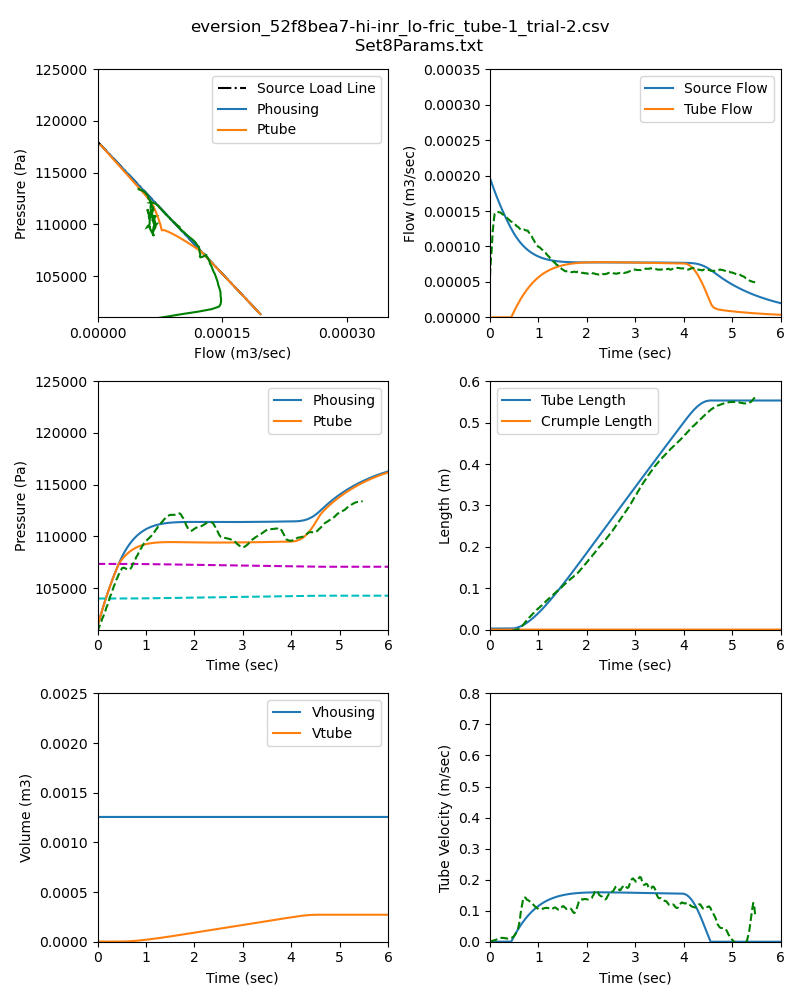
\includegraphics[width=0.475\textwidth]{Set8result27-Jul.png}
\caption{Simulation 8.}
\end{figure}


%  Use name of bibliography files without .bib extension
\bibliography{flowMOdel}
\end{document}
